\documentclass[twocolumn]{aastex631}
% generated by paper/make_inputs.py from results/*.json; do not edit
\newcommand{\fskyA}{0.92}
\newcommand{\fskyB}{0.60}
\newcommand{\netChiA}{28.8}
\newcommand{\netPteA}{0.12}
\newcommand{\netChiB}{30.7}
\newcommand{\netPteB}{0.08}
\newcommand{\chiDiff}{3.32}
\newcommand{\pteDiff}{0.85}
\newcommand{\nBoot}{2{,}000}
\newcommand{\maxPullMap}{143B}
\newcommand{\maxPull}{+0.70}
\newcommand{\pearsonR}{0.984}
\newcommand{\betaMK}{0.25}
\newcommand{\sigBetaMK}{0.23}
\newcommand{\betaProf}{0.25}
\newcommand{\sigBetaProf}{0.23}
\newcommand{\betaNoDust}{-0.08}
\newcommand{\sigBetaNoDust}{0.14}
\newcommand{\betaOneA}{0.09}
\newcommand{\sigBetaOneA}{0.18}
\newcommand{\betaAncA}{0.24}
\newcommand{\betaAncB}{0.23}
\newcommand{\sigBetaAnc}{0.23}
\newcommand{\dustRatioA}{1.41}
\newcommand{\dustRatioB}{1.40}
\newcommand{\dustRatioC}{1.40}
\newcommand{\spChiTw}{70.9}
\newcommand{\spDofTw}{77}
\newcommand{\spPteTw}{0.67}
\newcommand{\clChiTw}{245.9}
\newcommand{\clDofTw}{252}
\newcommand{\clPteTw}{0.60}
\newcommand{\abChiTw}{45.8}
\newcommand{\abDofTw}{44}
\newcommand{\abPteTw}{0.397}
\newcommand{\trChiTw}{6.3}
\newcommand{\trPteTw}{0.50}
\newcommand{\nullSpTw}{77.3}
\newcommand{\nullClTw}{252.5}
\newcommand{\nullAbTw}{44.0}
\newcommand{\powDustTw}{92}
\newcommand{\powInstTw}{90}
\newcommand{\spChiEi}{67.9}
\newcommand{\spDofEi}{49}
\newcommand{\spPteEi}{0.04}
\newcommand{\clChiEi}{171.2}
\newcommand{\clDofEi}{168}
\newcommand{\clPteEi}{0.42}
\newcommand{\abChiEi}{49.0}
\newcommand{\abDofEi}{28}
\newcommand{\abPteEi}{0.008}
\newcommand{\trChiEi}{8.5}
\newcommand{\trPteEi}{0.29}
\newcommand{\nullSpEi}{48.1}
\newcommand{\nullClEi}{168.4}
\newcommand{\nullAbEi}{28.0}
\newcommand{\powDustEi}{46}
\newcommand{\powInstEi}{84}
\newcommand{\nNull}{500}
\newcommand{\abBonf}{0.07}
\newcommand{\leakMean}{+0.002}
\newcommand{\leakMax}{0.078}
\newcommand{\leakFloor}{0.16}
\newcommand{\nzN}{+2.76}
\newcommand{\npN}{0.006}
\newcommand{\nhN}{0.08}
\newcommand{\nzS}{+2.16}
\newcommand{\npS}{0.034}
\newcommand{\nhS}{0.37}
\newcommand{\nzC}{+2.78}
\newcommand{\npC}{0.006}
\newcommand{\nhC}{0.08}
\newcommand{\nPers}{1{,}000}
\newcommand{\nComp}{13}
\newcommand{\asymZ}{-0.07}
\newcommand{\pvGNz}{+2.90}
\newcommand{\pvGNh}{0.07}
\newcommand{\pvGSz}{+2.19}
\newcommand{\pvGSh}{0.52}
\newcommand{\pvGCz}{+2.62}
\newcommand{\pvGCh}{0.25}
\newcommand{\pvANz}{+2.82}
\newcommand{\pvANh}{0.07}
\newcommand{\pvASz}{+2.08}
\newcommand{\pvASh}{0.95}
\newcommand{\pvACz}{+2.61}
\newcommand{\pvACh}{0.42}
\newcommand{\pvPNz}{+3.68}
\newcommand{\pvPNh}{0.07}
\newcommand{\pvPSz}{+3.00}
\newcommand{\pvPSh}{0.07}
\newcommand{\pvPCz}{+3.20}
\newcommand{\pvPCh}{0.13}
\newcommand{\nPV}{1{,}000}
\newcommand{\covF}{0.62}
\newcommand{\covnF}{0.91}
\newcommand{\bsdF}{0.63}
\newcommand{\covZ}{0.61}
\newcommand{\covnZ}{0.91}
\newcommand{\bsdZ}{0.70}
\newcommand{\mkBiasZ}{-0.092}
\newcommand{\mkCovZ}{0.23}
\newcommand{\covO}{0.60}
\newcommand{\covnO}{0.91}
\newcommand{\bsdO}{0.64}
\newcommand{\mkBiasO}{-0.072}
\newcommand{\mkCovO}{0.04}
\newcommand{\covT}{0.61}
\newcommand{\covnT}{0.90}
\newcommand{\bsdT}{0.63}
\newcommand{\mkBiasT}{+0.195}
\newcommand{\mkCovT}{0.04}
\newcommand{\covH}{0.57}
\newcommand{\covnH}{0.91}
\newcommand{\bsdH}{0.65}
\newcommand{\dcovF}{0.72}
\newcommand{\dsdF}{0.34}
\newcommand{\dcovZ}{0.79}
\newcommand{\dsdZ}{0.32}
\newcommand{\dcovO}{0.75}
\newcommand{\dsdO}{0.33}
\newcommand{\dcovT}{0.70}
\newcommand{\dsdT}{0.34}
\newcommand{\dcovH}{0.74}
\newcommand{\dsdH}{0.33}
\newcommand{\mkSlopeO}{+0.29}
\newcommand{\mkSlopeZ}{+0.18}
\newcommand{\nTest}{2{,}000}
\newcommand{\rwKH}{1.06}
\newcommand{\dcovnF}{0.97}
\newcommand{\rwCovH}{0.62}
\newcommand{\rwCovnH}{0.93}
\newcommand{\rwHwH}{0.43}
\newcommand{\rwCovO}{0.61}
\newcommand{\rwCovnO}{0.93}
\newcommand{\rwHwO}{0.59}
\newcommand{\fisNoDust}{0.149}
\newcommand{\fisFull}{\infty}
\newcommand{\fisEig}{\sim10^{-15}}
\newcommand{\npeBeta}{-0.01}
\newcommand{\npeUp}{0.83}
\newcommand{\npeLo}{0.83}
\newcommand{\npeLoN}{-1.34}
\newcommand{\npeHiN}{1.34}
\newcommand{\dOffset}{0.4}
\newcommand{\dBeta}{-0.09}
\newcommand{\dUp}{0.29}
\newcommand{\dLo}{0.28}
\newcommand{\bPsiH}{-0.07}
\newcommand{\bPsiHUp}{0.55}
\newcommand{\bPsiHLo}{0.52}
\newcommand{\bPsiO}{-0.03}
\newcommand{\bPsiOUp}{0.74}
\newcommand{\bPsiOLo}{0.72}
\newcommand{\bPsiT}{-0.02}
\newcommand{\bPsiTUp}{0.85}
\newcommand{\bPsiTLo}{0.84}


\shorttitle{Closure tests of the PR4 calibration network and the $\beta$--$\psi$ degeneracy}
\shortauthors{Zulu}

\begin{document}

\title{Region-resolved closure tests of the Planck PR4 polarization-angle calibration network and the exact degeneracy of birefringence with dust misalignment}

\author{Nomo Zulu}
\affiliation{Independent Researcher}

\begin{abstract}
Cosmic birefringence searches are limited by the absolute calibration of detector polarization
angles. \citet{lka2026} introduced a birefringence-blind differential test on the eight Planck PR4
(NPIPE) detector-split maps: pairwise angle differences form a network whose consistency with the
Minami--Komatsu (MK) calibration pattern can be checked without assuming foreground EB.
We present an independent implementation on the public maps. The 28 pair angles close
($\chi^2=\netChiA$ for 21 degrees of freedom) and agree with an MK fit of the same maps
($\chi^2_{\rm diff}=\chiDiff$ for 7 dof, PTE $\pteDiff$; Pearson $r=\pearsonR$), with the largest
pull at the same map the original analysis identified. We formulate the network as a cochain
complex on the filled complete graph $K_8$: the common rotation is the gauge kernel of the
coboundary, $H^1=0$, and the residual of the covariance-weighted fit is a weighted coexact
component whose quadratic form equals the triangle-closure statistic.
We then ask a question the global analysis cannot: is the calibration pattern the same across the
sky? Splitting the misfit exactly into within-region closure and a spatial-stationarity term,
with blinded, pre-registered thresholds, we find no evidence for spatial variation over twelve
equal-area regions ($\chi^2=\spChiTw$ for $\spDofTw$ dof, PTE $\spPteTw$), a test that detects a
$0.1^\circ$ instrument-like drift $\powInstTw\%$ of the time. A latitude-band partition shows a
hint of variation on the dust-immune same-frequency edges that does not survive correction for
the number of statistics reported.
Finally, a coverage-validated neural posterior estimator over a family of dust-EB models shows
that, once the dust misalignment $\psi$ is free, $\beta$ is exactly degenerate with it: these
channels measure $\beta-\psi_0=\dBeta^{+\dUp}_{-\dLo}$\,deg, and $\beta$ itself follows only from
an assumed prior on $\psi_0$ ($\beta=\bPsiH^{+\bPsiHUp}_{-\bPsiHLo}$\,deg for
$\psi_0\sim\mathcal N(0,0.5^\circ)$).
\end{abstract}

\keywords{cosmic background radiation --- polarization --- methods: data analysis}

\section{Introduction}
A parity-violating rotation of the CMB polarization plane by an angle $\beta$ would convert E-mode
into B-mode power and produce a nonzero EB correlation. Recent analyses of Planck, WMAP and ACT
data report $\beta\approx0.2^\circ$--$0.4^\circ$ \citep{mk2020,dp2022,ek2022,act2025}, but $\beta$
is exactly degenerate with a common rotation of all detector angles. The MK method
\citep{mk2019,mk2020} breaks the degeneracy by using Galactic foreground emission, which is rotated
by the instrument but not by $\beta$, at the cost of assumptions about the intrinsic EB of dust
\citep{clark2021}.

\citet{lka2026} proposed a complementary consistency test. For two maps $i,j$ rotated by
$\alpha_i,\alpha_j$, the antisymmetric and symmetric cross-spectra satisfy
\begin{equation}
C_\ell^{B_iE_j}-C_\ell^{E_iB_j}=\tan\!\big[2(\alpha_i-\alpha_j)\big]\,\big(C_\ell^{E_iE_j}+C_\ell^{B_iB_j}\big)
\end{equation}
for any sky EE, BB and intrinsic EB, so the common rotation cancels. The 28 pair angles of the
eight NPIPE detector-split maps reconstruct the relative calibration pattern, which can be
compared with the MK pattern on the seven-dimensional differential subspace.

This paper (i) independently implements the test on the public maps and quantifies agreement,
(ii) states the cochain structure of the network precisely, (iii) introduces a
region-resolved extension that tests whether the calibration pattern is spatially stationary,
with a dust-immune instrument control, (iv) quantifies with simulation-based inference what the
same channels can say about $\beta$ once the dust misalignment is free, and (v) reports a
topological diagnostic of the temperature map against noise-realistic and phase-randomized
nulls.

\section{Data and spectra}
We use the eight PR4 NPIPE detector-split maps at $N_{\rm side}=2048$ (100, 143, 217 and 353\,GHz,
splits A and B; each file header records its \texttt{npipe6v20A/B} source) \citep{npipe2020}.
The masks of \citet{lka2026} are not public; we rebuild them from Planck Legacy Archive products:
the union of the polarized point-source masks at 100--353\,GHz times a CO(2--1) cut chosen to
reach $f_{\rm sky}=\fskyA$, and the same times the PLA Galactic mask whose combination lands
nearest $f_{\rm sky}=0.62$ ($\fskyB$). Spin-2 harmonic transforms use \texttt{ducc0}
\citep{ducc}; all $16\times16$ field cross-spectra are binned in 72 bins of width 20 over
$51\le\ell<1491$. We divide pseudo-$C_\ell$ by $\langle w^2\rangle$ rather than deconvolving mode
coupling; pair angles are ratios and are insensitive to this, while for the MK theory term we
apply a mask transfer function measured from $\Lambda$CDM simulations. Beam windows are the NPIPE
QuickPol products.

\section{The network as a cochain complex}
Let maps be the vertices of $K_8$, pairs its 28 edges and fill all 56 triangles. With
$(d_0x)_{ij}=x_i-x_j$ and $(d_1w)_{ijk}=w_{ij}+w_{jk}-w_{ik}$, the pair-angle model is
$\Delta\alpha=d_0\alpha+n$, so the incidence matrix of \citet{lka2026} is the coboundary $d_0$, and
$\ker d_0=\mathrm{span}\{\mathbf 1\}$ is the common rotation (the gauge freedom they note). Since
$\mathrm{rank}\,d_0=7$ and $\mathrm{rank}\,d_1=21$, the first cohomology vanishes, $H^1=0$: no
harmonic component exists, and anything outside $\mathrm{im}\,d_0$ is a failure of triangle
closure.

The generalized least-squares fit with edge covariance $C$ is orthogonal in the $C^{-1}$ metric.
Its residual $r$ obeys $d_0^{\!\top}C^{-1}r=0$, so $C^{-1}r\in\mathrm{im}\,d_1^{\!\top}$: $r$ is a
\emph{covariance-weighted} coexact component, and need not lie in $\mathrm{im}\,d_1^{\!\top}$
itself unless $C$ preserves that subspace. The metric-free closures $d_1\Delta\alpha$ carry the
same information: their quadratic form $c^{\!\top}(d_1Cd_1^{\!\top})^{+}c$ equals the GLS residual
$\chi^2$ with 21 degrees of freedom. This graph ``curl'' is a calibration diagnostic, unrelated to
CMB B-modes. All numerical kernels are verified in a network-less sandbox with hash-chained
receipts (Appendix~\ref{app:vv}).

\section{Reproduction}
Pair angles come from a reweighted least-squares fit of Eq.~1 across bins with Gaussian bandpower
covariance propagated to the $28\times28$ pair covariance; their calibration was validated on
% typed value: 0.90 is from the local injection test (README), not in results/*.json
injected synthetic skies (pull standard deviation $0.90$). The gauge-fixed network fit gives
$\chi^2=\netChiA$ for 21 dof (PTE $\netPteA$) at $f_{\rm sky}=\fskyA$ and $\netChiB$ (PTE $\netPteB$) at
$f_{\rm sky}=\fskyB$. A numpy port of the MK likelihood of \citet{lka2026}, with four dust-EB
amplitudes, yields the per-map pattern of Fig.~\ref{fig:pattern}. Keeping the network--MK
cross-covariance from $\nBoot$ bootstrap draws of the bandpowers, $\chi^2_{\rm diff}=\chiDiff$
for 7 dof (PTE $\pteDiff$), compared with 8.18 (PTE 0.32) in \citet{lka2026}; the largest pull is
$\maxPullMap$ ($\maxPull\sigma$), the map they also single out. Dust $C_\ell^{EE}/C_\ell^{BB}$ at
$\ell<300$ is $\dustRatioA$, $\dustRatioB$ and $\dustRatioC$ at 143, 217 and 353\,GHz.

The MK birefringence angle is $\beta=\betaMK^\circ\pm\sigBetaMK^\circ$ (a profile likelihood
including $\ln\det C$ gives $\betaProf\pm\sigBetaProf$), consistent with $0.37^\circ\pm0.11^\circ$
\citep{lka2026} but with about twice the uncertainty. It depends on the dust-EB model:
$\betaNoDust\pm\sigBetaNoDust$ with no dust EB and $\betaOneA\pm\sigBetaOneA$ with one
amplitude, mirroring the known shift between dust treatments in PR4 \citep{dp2022}.

\begin{figure}
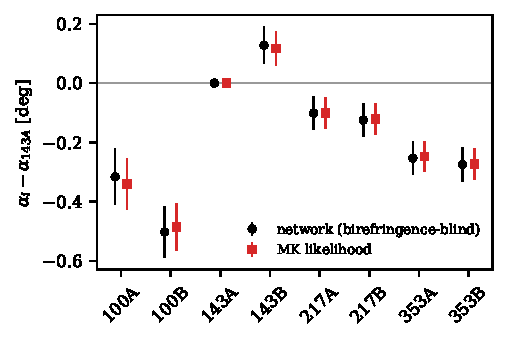
\includegraphics[width=\columnwidth]{figures/fig_pattern.pdf}
\caption{Per-map calibration pattern (gauge $\alpha_{143A}=0$) from the birefringence-blind
network and from the MK likelihood on the same maps.\label{fig:pattern}}
\end{figure}

\section{Is the calibration pattern spatially stationary?}
\subsection{Statistic}
We measure the 28 pair angles separately in $R$ disjoint regions with covariances $C_r$
(block-diagonal; map-level simulations give a mean cross-region correlation of $\leakMean$, maximum
$\leakMax$, against a noise floor of $\leakFloor$). With $F_r=A^{\!\top}C_r^{-1}A$ ($A=d_0$ without the
gauge column) the global-fit residual splits exactly,
\begin{equation}
\chi^2_{\rm total}=\sum_r\chi^2_{{\rm closure},r}+\sum_r(\hat\alpha_r-\hat\alpha)^{\!\top}F_r(\hat\alpha_r-\hat\alpha),
\end{equation}
with $21R$ and $7(R-1)$ degrees of freedom. The second term, $\chi^2_{\rm spatial}$, tests whether
the per-map pattern differs between regions. A sky-dependent \emph{common} rotation, such as
anisotropic birefringence, is gauge and invisible. The four same-frequency A/B edges compare
detectors in the same band, so foregrounds cancel; variation on them is instrumental.

\subsection{Blinding and validation}
Validation used each region's real spectra with the antisymmetric part removed after derotating
by the published global angles, so no regional pair angle was formed before the analysis was
frozen. Code hashes, statistic definitions and the threshold (PTE$<0.01$; twelve HEALPix base
pixels primary, eight latitude bands as a robustness partition) were committed before a single
unblinding run. On $\nNull$ null skies the statistics match their degrees of freedom (mean
$\chi^2_{\rm spatial}=\nullSpTw$ for $\spDofTw$ dof; closure $\nullClTw$ for $\clDofTw$). The
twelve-region test detects a $0.2^\circ$ dust-like drift $\powDustTw\%$ and a $0.1^\circ$
instrument-like drift $\powInstTw\%$ of the time.

\subsection{Result}
For twelve regions $\chi^2_{\rm spatial}=\spChiTw$ for $\spDofTw$ dof (PTE $\spPteTw$), closure
$\clChiTw$ for $\clDofTw$ (PTE $\clPteTw$), A/B edges $\abChiTw$ for $\abDofTw$ (PTE $\abPteTw$) and no
dependence on a 353\,GHz dust tracer ($\Delta\chi^2=\trChiTw$ for 7, PTE $\trPteTw$;
Fig.~\ref{fig:spatial}). The calibration pattern is spatially stationary at this sensitivity.
In the latitude partition $\chi^2_{\rm spatial}=\spChiEi$ for $\spDofEi$ (PTE $\spPteEi$) and the A/B
edges give $\abChiEi$ for $\abDofEi$ (PTE $\abPteEi$), driven by the 143\,GHz pair and the northern
$20^\circ$--$40^\circ$ band in a pattern consistent with a shift of one map; over the eight
statistics reported the Bonferroni-corrected value is $\abBonf$. We report it as a target for
split-based follow-up rather than a detection.

\begin{figure*}
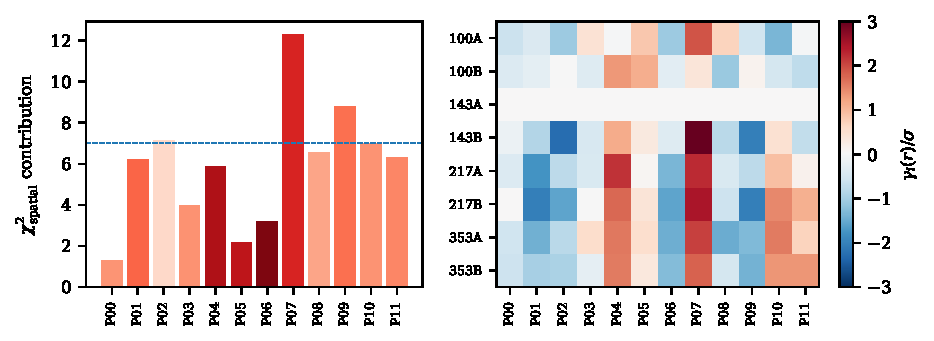
\includegraphics[width=\textwidth]{figures/fig_spatial.pdf}
\caption{Left: per-region contributions to $\chi^2_{\rm spatial}$ (expected 7 each; darker bars carry
more 353\,GHz dust). Right: regional drift $\gamma_i(r)$ of each map in units of its error (gauge
143A).\label{fig:spatial}}
\end{figure*}

\section{What the HFI channels say about $\beta$}
\subsection{Simulation-based inference}
The MK estimate of $\beta$ moves with the dust-EB model (Sect.~4). To quantify this without
committing to one dust model, we train a neural posterior estimator. A bandpower simulator draws
exact Wishart realizations of the 136 field spectra per bin from: the $\Lambda$CDM spectra
(QuickPol windows, mask transfer) rotated by $\alpha_i+\beta$; a modified-blackbody dust component
scaled from the measured 353\,GHz spectra, whose polarization in band $i$ is intrinsically rotated
by a misalignment $\psi_i=\psi_0(\ell/200)^{n}+\psi_1\ln(\nu_i/353\,{\rm GHz})$, so that the
$(E_i,B_j)$ dust block is $R(\psi_i)\,{\rm diag}(C^{EE}_{\rm dust},C^{BB}_{\rm dust})\,R(\psi_j)^{\rm T}$
(for $\psi_i=\psi_j$ this is the familiar $C^{EB}_{\rm dust}=\frac{1}{2}\sin4\psi\,(C^{EE}_{\rm dust}-C^{BB}_{\rm dust})$,
and for $\psi_i\neq\psi_j$ it mimics a calibration difference); and the measured noise. This
family contains no dust EB, a constant misalignment, scale dependence and frequency dependence.
The angles $\alpha_i$ carry a broad common offset, $\mathcal U(-3^\circ,3^\circ)$; a narrow one
would let the prior, rather than the data, fix $\beta$. Summaries are the 14 scores at a fiducial
point, and an ensemble of five conditional masked autoregressive flows is trained on $4\times10^5$
simulations. The network's log-densities are recomputed in float64 in the verification sandbox.

\subsection{Validation}
On $\nTest$ held-out simulations per dust model, the 68\% and 95\% intervals for $\beta$ cover the
truth $\covF$ and $\covnF$ of the time for the full model (Fig.~\ref{fig:coverage}). The posterior
is wide, $\sigma_\beta\simeq\bsdF^\circ$, and a Fisher analysis at the fiducial point shows why:
$\sigma_\beta=\fisNoDust^\circ$ with no dust EB, but $\sigma_\beta=\fisFull$ once a constant
misalignment is free. Dust appears rotated by $\alpha+\psi$
and the CMB by $\alpha+\beta$, so a common shift of $\alpha$, $\beta$ and $\psi$ leaves the model
unchanged; numerically, the Fisher matrix has a single null direction,
$\delta\alpha_i=-\epsilon$ for all $i$ and $\delta\beta=\delta\psi_0=\epsilon$ (relative
eigenvalue $\fisEig$). The data constrain $\beta-\psi$ and $\alpha+\beta$, and $\beta$ alone is set by the
priors. Its marginal posterior is then a flat box bounded by prior edges, which the flows
represent imperfectly; this is the origin of the mild under-coverage of $\beta$ alone. The
identifiable combination $\beta-\psi_0$ is recovered with $\sigma\simeq\dsdF^\circ$ and coverage
$\dcovF$ (68\%) and $\dcovnF$ (95\%). For $\beta$ under an external prior on $\psi_0$, obtained by
importance re-weighting, we test calibration on simulations drawn from that prior: for
$\psi_0\sim\mathcal N(0,0.5^\circ)$ the intervals cover $\rwCovH$ (68\%) and $\rwCovnH$ (95\%), and for
$\mathcal N(0,1^\circ)$ $\rwCovO$ and $\rwCovnO$. Before unblinding we therefore fixed an empirical
calibration: each reported interval is widened about its median by the factor that restores
nominal coverage on these simulations ($\rwKH$ at 68\% for $\mathcal N(0,0.5^\circ)$), never
narrowed. For comparison, an MK fit without a dust-EB term
covers the truth only $\mkCovO$ of the time when a constant misalignment is present, and even
without dust EB its $\beta$ error grows with the absolute common miscalibration (slope
$\mkSlopeZ$ per degree), an attenuation from noise in the observed $C^{EE}$ that acts as its
regressor.

\begin{figure}
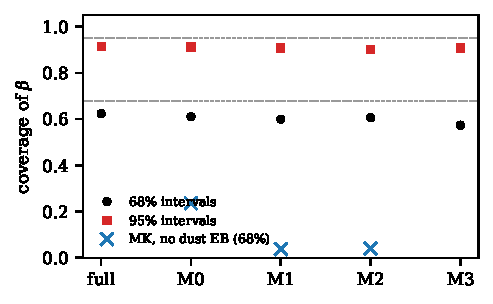
\includegraphics[width=\columnwidth]{figures/fig_coverage.pdf}
\caption{Coverage of $\beta$ by the neural posterior for each dust-EB model, and by an MK fit
without a dust-EB term (68\%).\label{fig:coverage}}
\end{figure}

\subsection{Result}
Applied once to the real spectra after a committed freeze, the posterior gives
$\beta-\psi_0=\dBeta^{+\dUp}_{-\dLo}$\,deg (68\%, calibrated), consistent with our MK fit without dust EB, which
measures the same combination. With no assumption on $\psi_0$, the $\beta$ posterior returns the
prior ($\npeBeta^{+\npeUp}_{-\npeLo}$\,deg). Re-weighting to a prior
$\psi_0\sim\mathcal N(0,0.5^\circ)$ gives $\beta=\bPsiH^{+\bPsiHUp}_{-\bPsiHLo}$\,deg. A precise
$\beta$ from these channels therefore requires an assumption about the mean dust misalignment, and
the published shift between dust treatments \citep{dp2022} is the expression of this degeneracy.
Our $\beta-\psi_0$ lies $\dOffset^\circ$ below the published no-dust-EB PR4 value of $0.30^\circ$
\citep{dp2022}; we attribute
this to pipeline differences (masks, pseudo-$C_\ell$) that we cannot resolve without the original
spectra.

\section{A topological diagnostic of the temperature map}
Sublevel persistent homology \citep{coleshiu2018} of three $20^\circ$ patches of the 143\,GHz
$(A+B)/2$ temperature map ($10'$ smoothing, $\ell\le1000$) at the Galactic caps and the Cold Spot
was compared with three null ensembles of $\nPV$ realizations each: isotropic Gaussian skies from
the measured masked-sky spectrum; Gaussian CMB plus anisotropic white noise with Planck's
per-pixel variance; and phase-randomized surrogates that keep the harmonic amplitudes of the
masked map exactly. Monte Carlo $p$-values carry the $+1$ correction and are Holm-adjusted over all
comparisons. The number of $H_0$ features is high against every null in all three patches:
Gaussian $z=\pvGNz$, $\pvGSz$, $\pvGCz$ (NGP, SGP, Cold Spot); with anisotropic noise $\pvANz$,
$\pvASz$, $\pvACz$; and against the phase surrogates $\pvPNz$, $\pvPSz$, $\pvPCz$. The smallest
Holm-adjusted $p$ is $\pvPNh$, the floor set by the number of realizations. Building the surrogates
from the unmasked map instead appears to remove the excess, but only because excluded
Galactic-plane power then enters them; masking the real patches instead cuts compact-source holes
into them that act as deep minima. None of these nulls reproduces the excess, though with Holm
$p\geq0.07$ none is excluded either. The leading candidate is the compact sources (and clusters) that the mask
flags inside the patches and that no null contains; a source-masked or source-injected null is the
next test. We report it as an unexplained diagnostic and claim no cosmological interpretation.

\section{Limitations}
Masks are rebuilt rather than identical to those of \citet{lka2026}; pseudo-$C_\ell$ replaces
NaMaster deconvolution; Fisher scoring replaces MCMC; covariances are Gaussian. The spatial test is
blind to anisotropic birefringence by construction, and regions are coarse (seven parameters per
region). The A/B edge-constancy statistic treats the four same-frequency edges as independent
within a region. A post-hoc check that keeps their full within-region covariance finds
correlations $|\rho|\le0.024$ and leaves the statistics essentially unchanged (latitude bands
% typed values: 0.024, 49.3, 49.0 are from the post-hoc audit (scripts/audit_spatial_ab.py), which writes outside the repo by design
$\chi^2=49.3$ for 28 dof instead of 49.0), but correlations between regions and uncertainty in the
covariance itself are not modelled. None of the analyses here uses end-to-end NPIPE simulations.

\section{Conclusions}
The differential calibration network of \citet{lka2026} reproduces on the public PR4 maps with an
independent pipeline. Its cochain structure makes the gauge, the absence of harmonic modes and the
equivalence of closure and fit $\chi^2$ explicit, and it extends naturally to a region-resolved
test, under which the Planck calibration pattern is spatially stationary within the sensitivity
stated above. A coverage-validated neural posterior shows that, with the dust misalignment free,
$\beta$ is exactly degenerate with it: these channels measure $\beta-\psi_0$, and any value of
$\beta$ quoted from them carries an assumption about $\psi_0$. Separating the two needs
information that does not rotate with the dust, such as an absolute calibrator or a measured
dust misalignment.

\section*{Data and code availability}
Code, results, verification receipts and an interactive summary are public at
\url{https://github.com/ZuluYokohama/cmb-cst-lab}. The MK likelihood is a port of the MIT-licensed
pipeline of \citet{lka2026}. Planck PR4 data are available from NERSC and the Planck Legacy Archive.

\begin{acknowledgments}
Based on observations obtained with Planck, an ESA science mission. Analysis code was developed
with the assistance of an AI coding assistant (Claude, Anthropic); the author is responsible for
the analysis and its conclusions.
\end{acknowledgments}

\appendix
\section{Verification}\label{app:vv}
Numerical kernels (network algebra, pair-angle estimator, MK likelihood, region statistics,
bootstrap kernels and persistence) are numpy-only and executed in a network-less container with
hash-chained receipts; GPU and NPU outputs are recomputed there in float64. Receipt identifiers are
listed in the repository README.

\begin{thebibliography}{}
\bibitem[{Lonappan} et al.(2026)]{lka2026} Lonappan, A.~I., Keating, B., \& Arnold, K. 2026, ApJL, 1009, L12 (arXiv:2609.09149)
\bibitem[{Minami} et al.(2019)]{mk2019} Minami, Y., Ochi, H., Ichiki, K., et al. 2019, PTEP, 2019, 083E02
\bibitem[{Minami} \& {Komatsu}(2020)]{mk2020} Minami, Y., \& Komatsu, E. 2020, PRL, 125, 221301
\bibitem[{Diego-Palazuelos} et al.(2022)]{dp2022} Diego-Palazuelos, P., Eskilt, J.~R., Minami, Y., et al. 2022, PRL, 128, 091302
\bibitem[{Eskilt} \& {Komatsu}(2022)]{ek2022} Eskilt, J.~R., \& Komatsu, E. 2022, PRD, 106, 063503
\bibitem[{ACT Collaboration}(2025)]{act2025} ACT Collaboration 2025, arXiv:2509.13654
\bibitem[{Clark} et al.(2021)]{clark2021} Clark, S.~E., Kim, C.-G., Hill, J.~C., \& Hensley, B.~S. 2021, ApJ, 919, 53
\bibitem[{Planck Collaboration}(2020)]{npipe2020} Planck Collaboration Int. LVII 2020, A\&A, 643, A42
\bibitem[{Cole} \& {Shiu}(2018)]{coleshiu2018} Cole, A., \& Shiu, G. 2018, JCAP, 2018, 025 (arXiv:1712.08159)
\bibitem[{Reinecke}(2023)]{ducc} Reinecke, M. 2023, ducc0, \url{https://gitlab.mpcdf.mpg.de/mtr/ducc}
\end{thebibliography}

\end{document}
